\chapter{CMS coordinate system}
The CMS coordinate system (Fig.~\ref{fig:cms_coords}) takes the $z$ axis to be along the beamline and the origin at the collision point. 
The $x$ axis points to the center of the LHC and the $y$ axis is orthogonal to the $x$-$z$ plane. 
The $x$-$y$ plane defines the ``transverse'' plane, wherein quantities like transverse momentum \pt are measured. 
Naturally, cylindrical coordinates $(r,z,\phi)$ are used frequently, where $r$ is the transverse distance from the $z$-axis to any point in space and $\phi$ is the azimuthal angle. 
The pseudorapidity $\eta$ is often used in place of the polar angle $\theta$, where $\eta$ is defined as
\begin{equation}
    \eta \equiv -\ln{\bigg[\tan\bigg(\frac{\theta}{2}\bigg)\bigg]}
\end{equation}
That is, $\eta$ is zero in the transverse plane, and it approaches infinity along either direction of the beamline. 
It is preferred over $\theta$ because differences in $\eta$ are uniquely Lorentz-invariant under boosts along the $z$ axis, which is important in the context of proton-proton collisions, where the interacting partons will carry some random fraction of the proton's energy according to the parton distribution function. 
Moreover, since the pseudorapidity is simply a function of $\theta$, which is easily measured, it is preferred over the actual rapidity, which is a function of the particle's energy. 
However, the pseudorapidity of a particle is approximately equal to the rapidity, so long as its rest mass is much smaller than the magnitude of its momentum. 

\begin{figure}[htb]
    \centering
    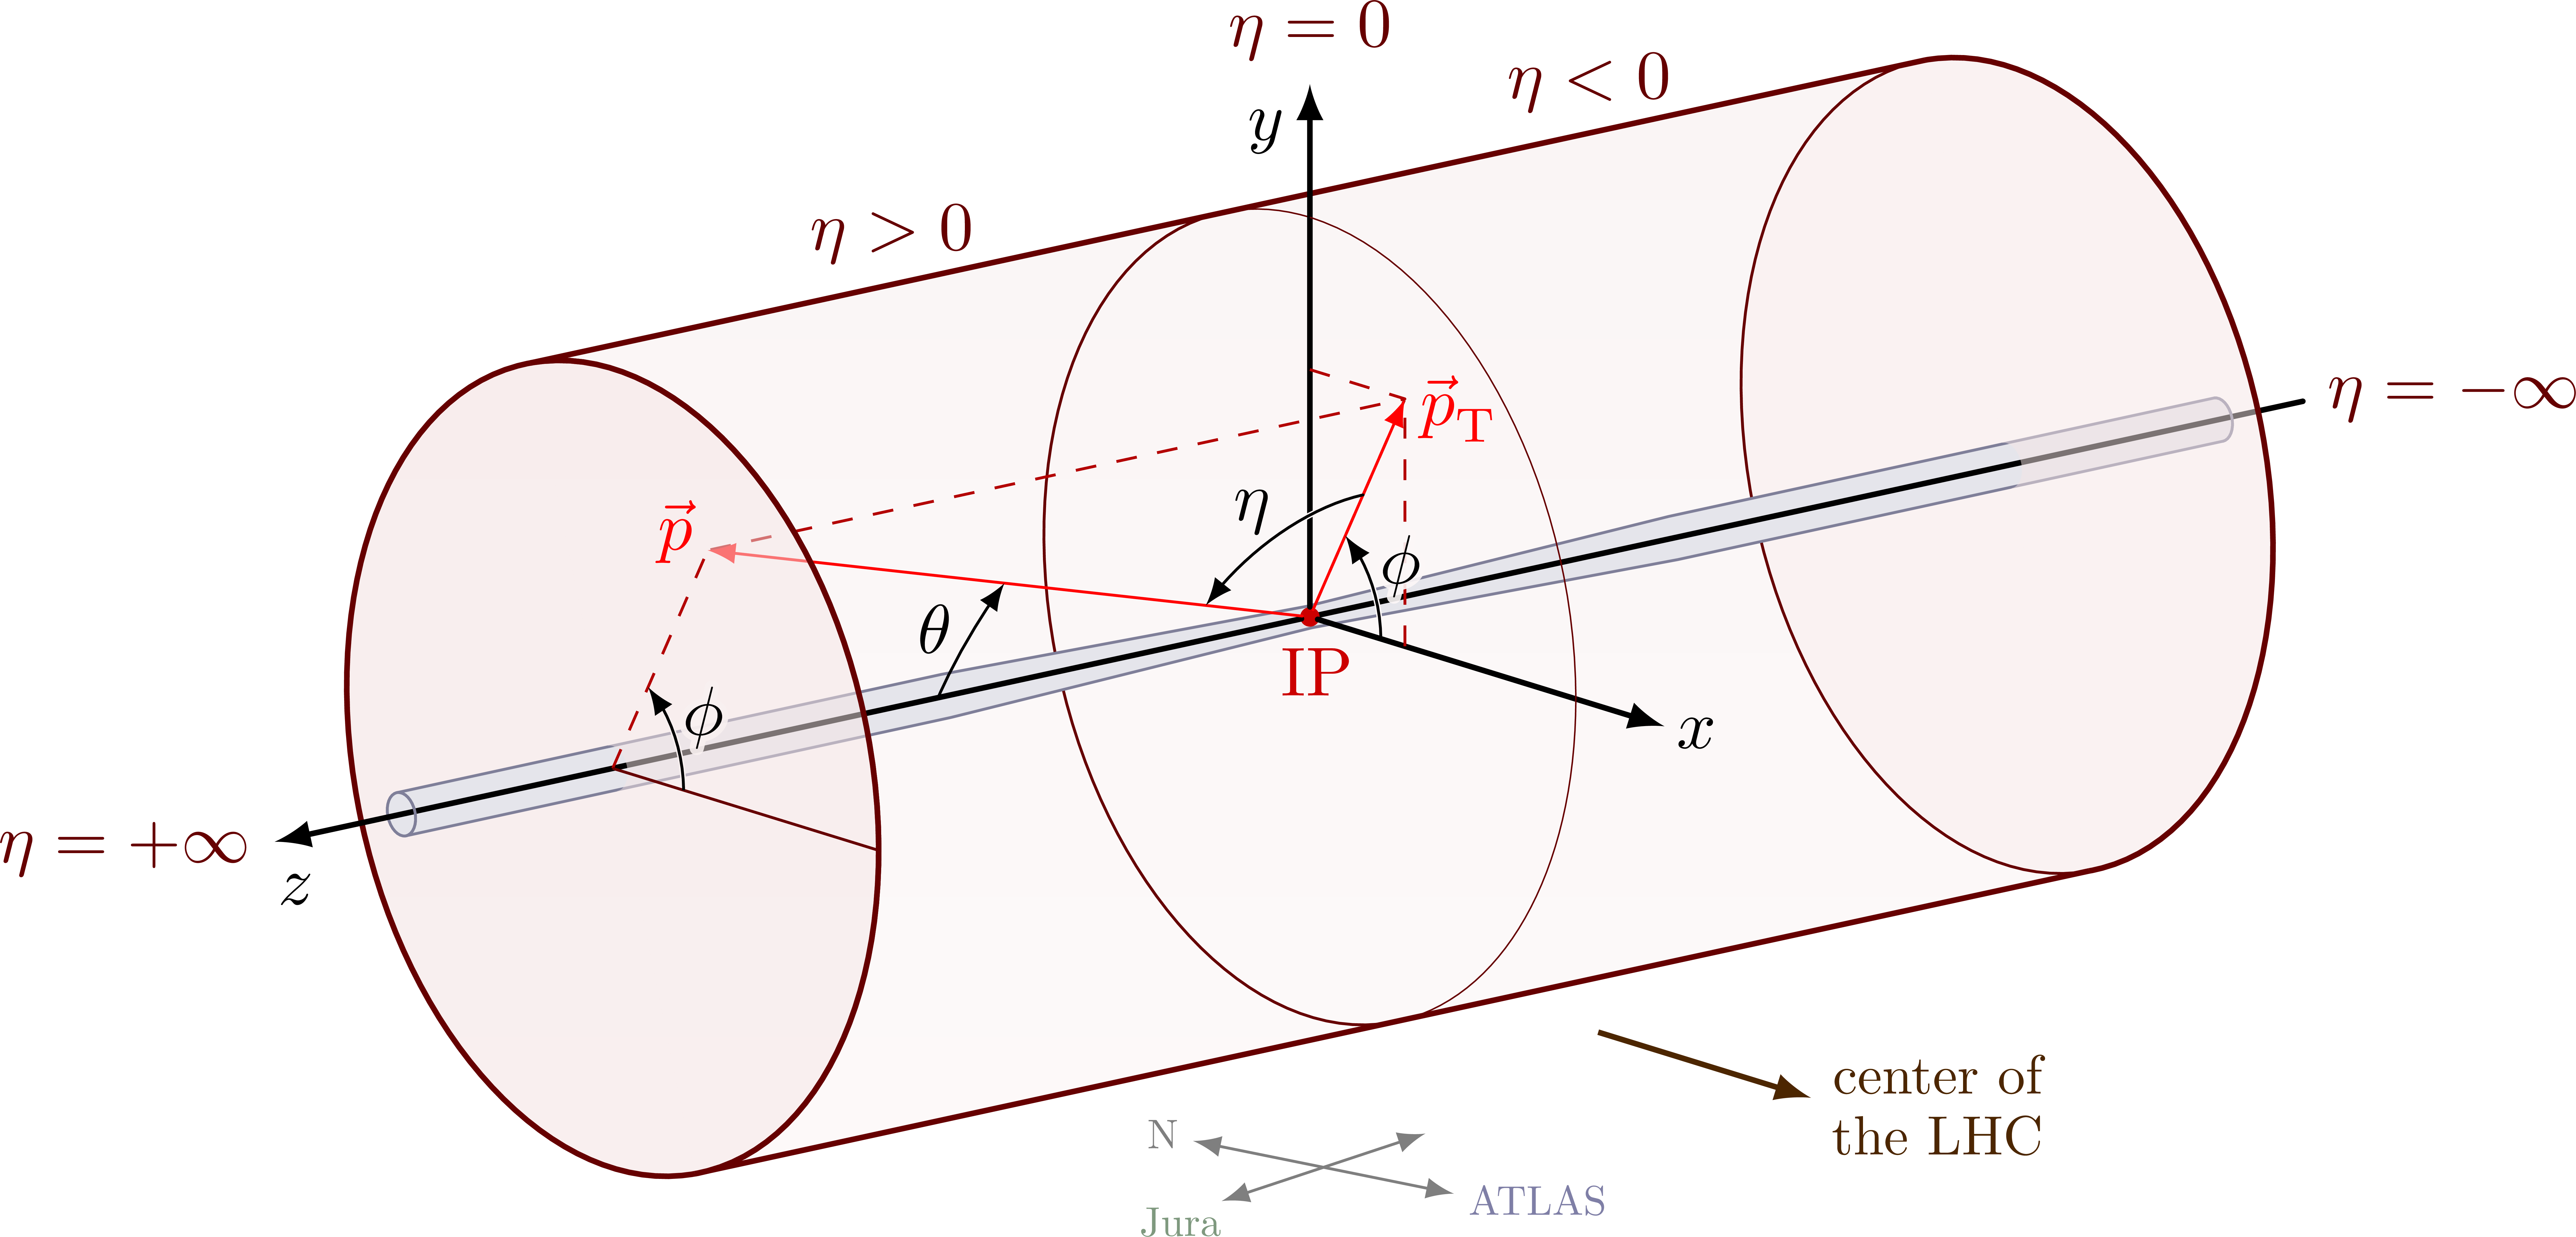
\includegraphics[width=0.8\textwidth]{fig/cms/coord_system.png}
    \caption[The CMS coordinate system]{
        The CMS coordinate system, from Ref~\cite{CMSCoords}, with a cylinder representing the volume of the CMS detector. 
    }
    \label{fig:cms_coords}
\end{figure}
